\documentclass[aspectratio=169]{beamer}
% \documentclass[aspectratio=169]{beamer} % proyector 16:9 | Ref:  https://en.wikibooks.org/wiki/LaTeX/Presentations
\usetheme{Boadilla}
\beamertemplatenavigationsymbolsempty %% Sin barra navegación
\usecolortheme{beaver}

\defbeamertemplate{footline}{special footline}{%
  %special footline
}

%% EDIT from me: In my case it worked, when I changed \setbeamertemplate
%% to \defbeamertemplate
%\setbeamertemplate{footline}{%
\defbeamertemplate{footline}{%
  normal footline
}


\makeatletter
\def\ps@navigation@titlepage{%
%% EDIT from me: the second braces need to be optional braces
%  \setbeamertemplate{footline}{special footline}
  \setbeamertemplate{footline}[special footline]
  \@nameuse{ps@navigation}
}
\addtobeamertemplate{title page}{\thispagestyle{navigation@titlepage}}{}
\makeatother

\AtBeginSection[]{%
\begingroup
%% EDIT from me: again, there need to be optional braces
%\setbeamertemplate{footline}{special footline}
\setbeamertemplate{footline}[special footline]
\begin{frame}
  \sectionpage
\end{frame}
\endgroup
}

\apptocmd{\tableofcontents}{\thispagestyle{navigation@titlepage}}{}{}


%% Spanska!
\usepackage[utf8]{inputenc}
\usepackage{lmodern} % no producia letras en matemático | Ref: https://tex.stackexchange.com/questions/250413/error-when-using-greek-symbol-in-subscript-in-beamer-presentation
\usepackage[spanish]{babel}
\def\spanishoptions{argentina}

%% inclusión de gráficas
\usepackage{graphicx}	% instalar ghostscript-x para que el dvi muestre los eps
\graphicspath{ {./graphs/} {../figuras/} {../unlam_mep2023/graphs/}}
\usepackage{rotating}	% epígrafe rotado


\begin{document}

\title[A code centred mechanics subject]{A rational mechanics course where everything\\is made with Python code}
% \subtitle{Capitalizando lo desarrollado durante el confinamiento}
\author[vbettachini@unlam.edu.ar]{Bettachini, Víctor A.\textsuperscript{1} Real, Mariano A.\textsuperscript{1} Palazzo, Edgardo\textsuperscript{2}}
\institute[]{
	
\includegraphics[height= 0.05\textwidth]{ambos}
	
\includegraphics[height= 0.05\textwidth]{Logo-UTN-Header}\\
	\textsuperscript{1} DIIT, Universidad Nacional de La Matanza, \textsuperscript{2} FRA, Universidad Tecnológica Nacional, ARGENTINA
}
\date[2023-11-23]{
	New Media Pedagogy 23\\Research trends, methodological challenges\\and succesful implementations\\
	21-24 november 2023\\ \vspace{0.2cm} 
\includegraphics[height= 0.06\textwidth]{logos}
	% 
\includegraphics[width= 0.3\textwidth]{logos}
}

%\usebackgroundtemplate{
%  
\includegraphics[width=\paperwidth, height=\paperheight]{diit_titre_background}
%}	% unset background % https://tex.stackexchange.com/questions/201013/how-to-include-a-background-image-to-only-one-page-of-a-beamer-presentation


\begin{frame}
  \titlepage
\end{frame}



%\usebackgroundtemplate{
%  
\includegraphics[width=\paperwidth, height=\paperheight]{diit_background}
%} %% https://mprnotes.wordpress.com/2009/08/14/changing-background-image-of-latex-beamer/


\begin{frame}
	\frametitle{Value student's and professor's time}
	Licklider (1957): 85\% of ``thinking'' are actually mundane tasks (calculations, drawings, etc.)
	\pause
	\begin{block}{}
	  \begin{columns}[b]
			\begin{column}{0.25\textwidth}
				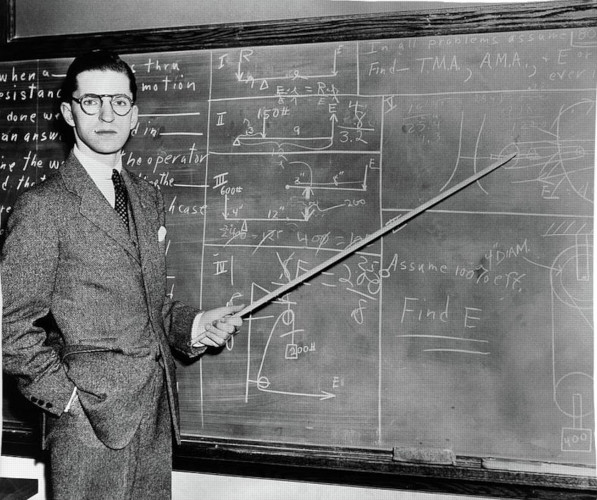
\includegraphics[width= \columnwidth]{1930s-1940s-man-teacher-professor-vintage-images}
			\end{column}
			\begin{column}{0.65\textwidth}
				Most current classrooms: an excercise on transcription
				\begin{itemize}[<+->]
					\item Professor: prepares lessons \(\xrightarrow{by\, heart}\) blackboard/slides
					\item Student: blackboard/slides \(\xrightarrow{transcribes}\) own notebooks
					\item Assignments: do \textbf{again} same calculations, drawings,...
					\item Boredom \(\rightarrow \) loss of concentration on the subject
				\end{itemize}
			\end{column}
		\end{columns}
	\end{block}
	\pause
	\begin{block}{}
	  \begin{columns}[b]
			\begin{column}{0.25\textwidth}
				\includegraphics[width= \columnwidth]{"Screenshot 2023-09-18 at 12-24-03 Google Colaboratory"}
			\end{column}
			\begin{column}{0.65\textwidth}
				Digital course material with embedded code
				\begin{itemize}[<+->]
					\item Professor: ideas \(\xrightarrow{updates}\) code/theory in repository
					\item Student: course repository \(\xrightarrow{clones}\) its own modifiable one
					\item \textbf{Recycles} professor's code to solve new problems
					%\item Modifiying it solves different problems
				\end{itemize}
			\end{column}
		\end{columns}
	\end{block}
\end{frame}



\begin{frame}
	\frametitle{Engineering students can take advantage of code at every single lecture}
	\pause
	\begin{block}{}
		\begin{itemize}[<+->]
			\item Currently they use a pocket calculator \textbf{after they learnt} arithmetics at school
			\item Now they'll employ computational algebra \textbf{after they learnt} algebra and calculus
			\begin{itemize}[<+->]
				\item Focus on new skills, not in automatable calculations
				%\item Álgebra y análisis simbólico
				\item Employing numerical calculus they solve what is impossible in a blackboard/paper
			\end{itemize}
			\end{itemize}
		% \uncover<4->{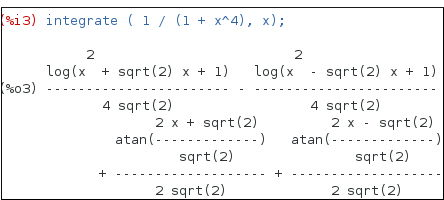
\includegraphics[height= 2cm]{ucarecdn}}
	\includegraphics[height= 2.5 cm]{reglacalculadora}
	\uncover<3->{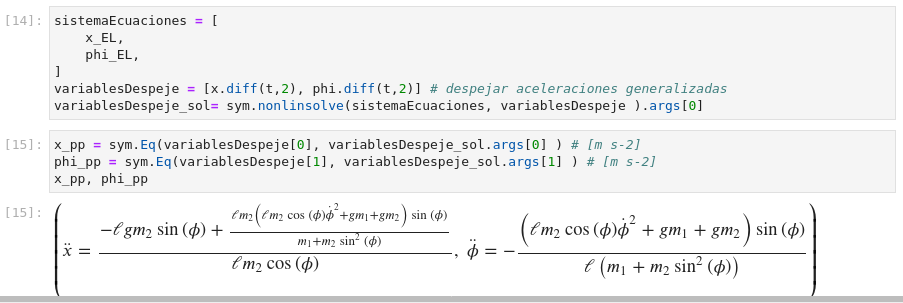
\includegraphics[height= 3.5 cm]{hard}}
	% \uncover<5->{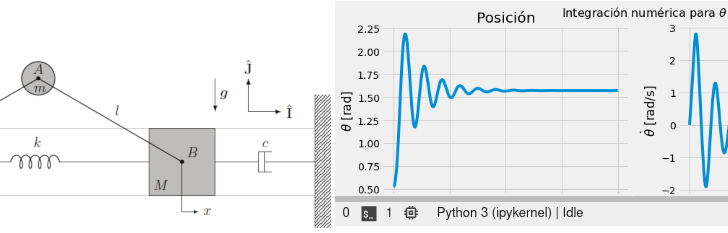
\includegraphics[width= 0.49\textwidth]{impracticable}}
	\end{block}
\end{frame}


\begin{frame}
	\frametitle{Engineering students can take advantage of code at every single lecture}
	\pause
	\begin{block}{}
		Papert (1980) ``...the best learning takes place when the learner takes charge''
		\begin{itemize}[<+->]
			\item An example problem is solved by the professor provided code
			\item The student \textbf{recycles} it to solve other related problems
			\item Gradually becoming autonomous by reusing not the provided but his own code
		\end{itemize}
	\end{block}
\end{frame}





\begin{frame}
	\frametitle{Tools | Jupyter notebook: text + equations + executable code}
	%\pause
	\begin{block}{}
	% \begin{block}{On-line programmable notebook: text + equations + code}
		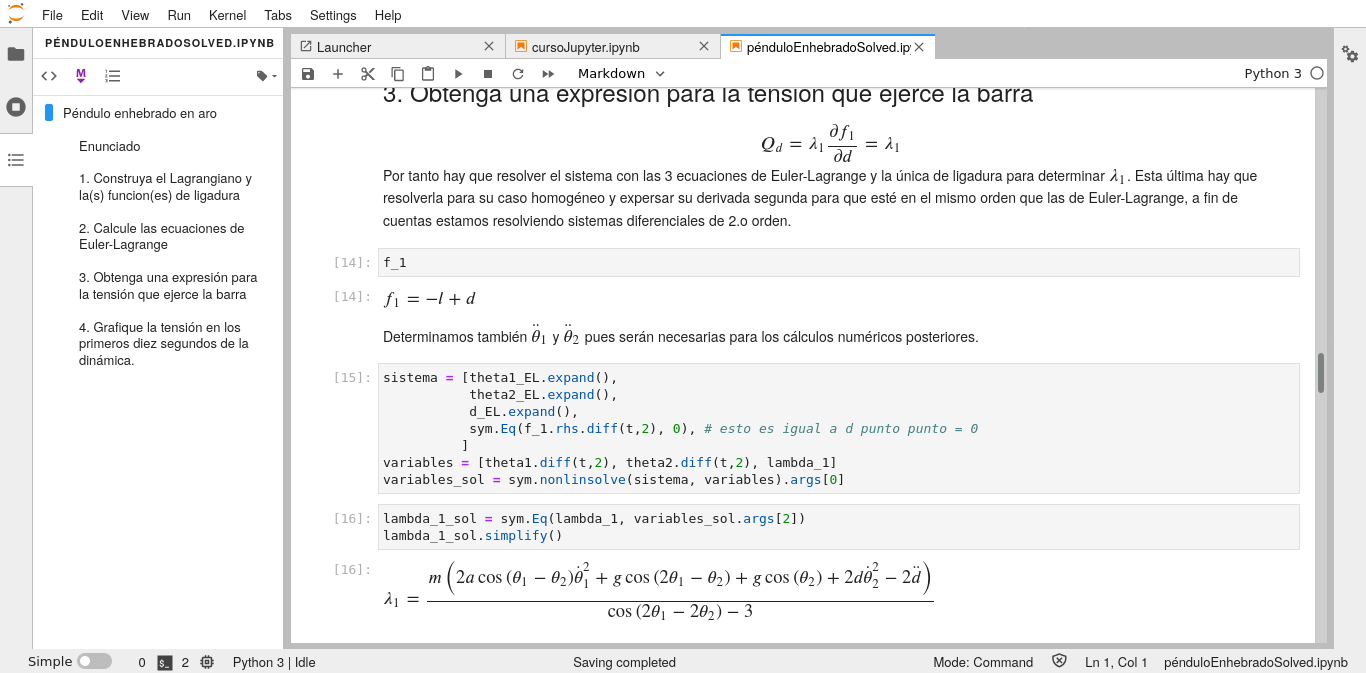
\includegraphics[width= \columnwidth]{screenshot_JupyterLab}
	\end{block}
\end{frame}




\begin{frame}
	\frametitle{Tools | Google Colaboratory runs Jupyter notebooks on-line}
	% \pause
	\begin{block}{}
		% \begin{itemize}[<+->]
		\begin{itemize}
			\item The platform allows professors to edit and comment on the work of students.
			% \item It runs Jupyter notebooks online, and it's free.
			\item Students can collaborate remotely, working on the same Jupyter notebook.
		\end{itemize}
		% \uncover<4->{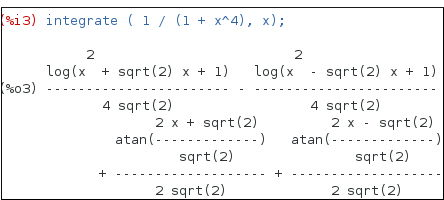
\includegraphics[height= 2cm]{ucarecdn}}
	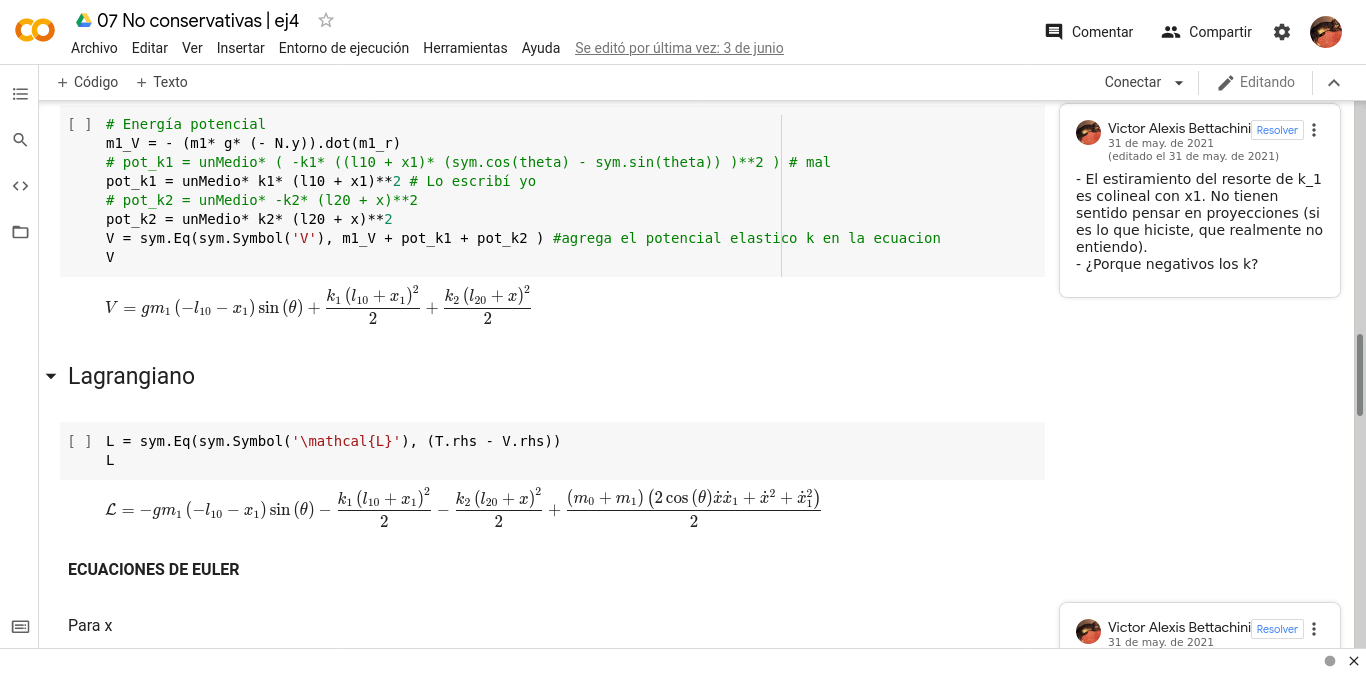
\includegraphics[width= 0.8\textwidth]{comentariosColab}
	\end{block}
	% \pause
\end{frame}


\begin{frame}
	\frametitle{Tools | All course material in a GitHub repository}
	% \pause 
	\begin{block}{}
		% \begin{itemize}[<+->]
		\begin{itemize}
			\item Clearly organised, freely accessible, and easy to update.
			\item Google Colaboratory loads Jupyter notebooks directly from GitHub.
		\end{itemize}
		% \uncover<4->{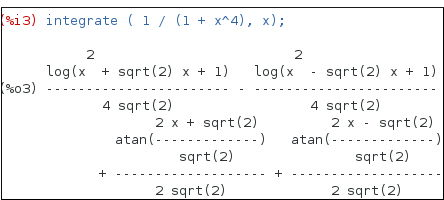
\includegraphics[height= 2cm]{ucarecdn}}
	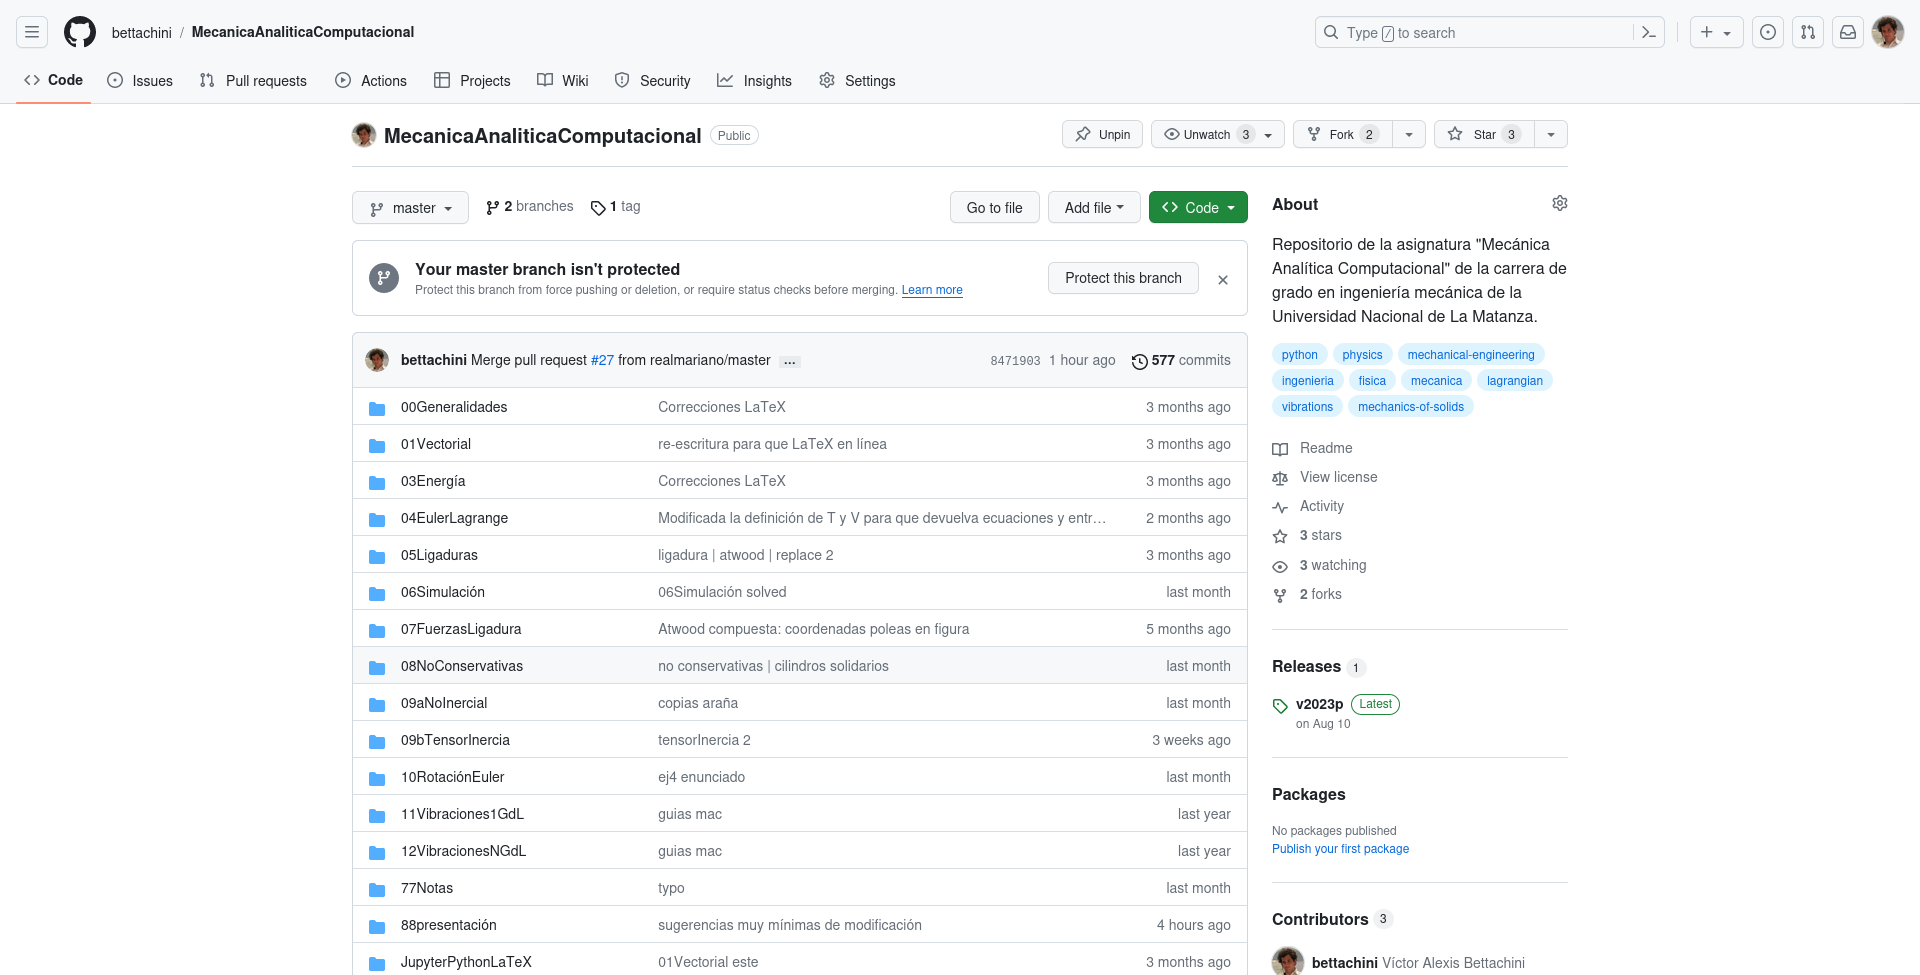
\includegraphics[width= \textwidth]{repositorioGithub}
	\end{block}
	% \pause
\end{frame}


\begin{frame}
	\frametitle{Tools | From the 1st class | \LaTeX \,: concise mathematical notation}
	% \pause
	\begin{block}{}
		\begin{itemize}
			\item \LaTeX \, typesetting follows strictly the standards of the American Mathematical Society
		\end{itemize}
		% \uncover<4->{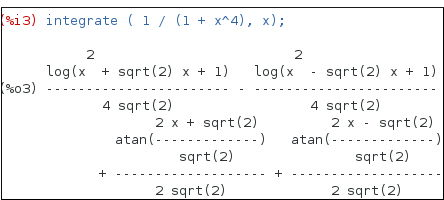
\includegraphics[height= 2cm]{ucarecdn}}
	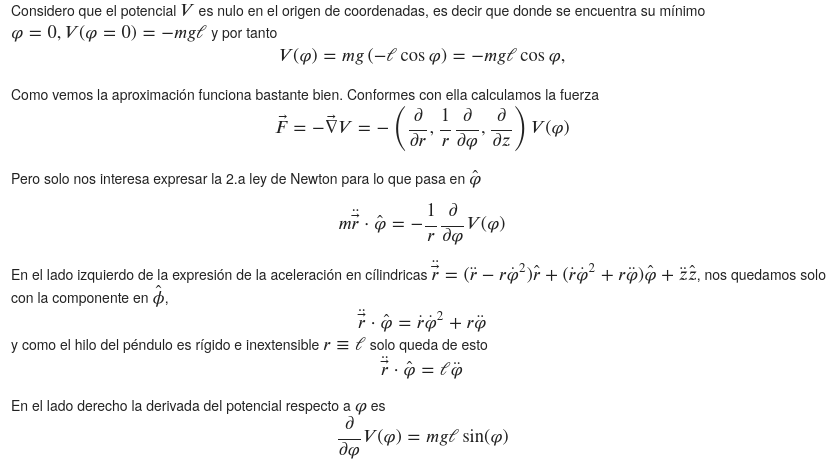
\includegraphics[width= 0.8\textwidth]{clase1péndulo}
	\end{block}
	% \pause
\end{frame}


\begin{frame}
	\frametitle{Tools | 1st class | Matplotlib: precise and reproducible graphics}
	% \pause
	\begin{block}{}
		\begin{itemize}
			\item Explicit Python code for producing graphics. Students are enticed to play with it.
		\end{itemize}
		% \uncover<4->{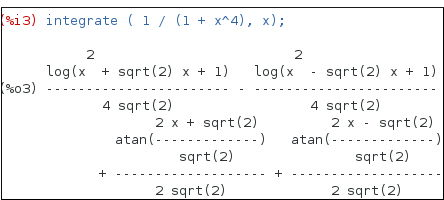
\includegraphics[height= 2cm]{ucarecdn}}
	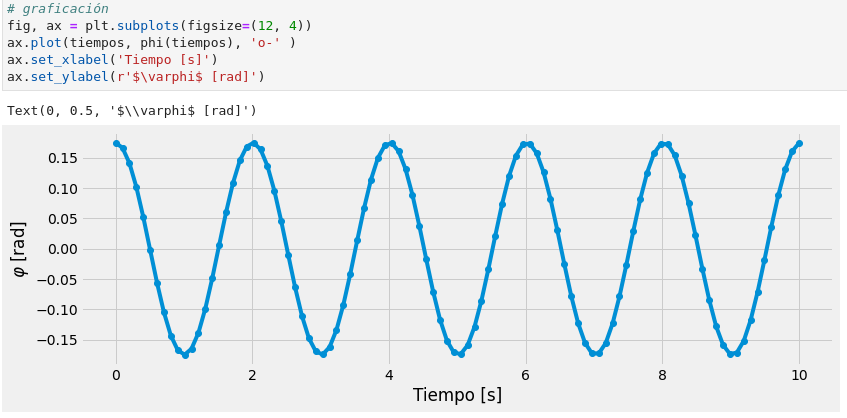
\includegraphics[width= 0.8\textwidth]{clase1gráficos}
	\end{block}
	% \pause
\end{frame}


\begin{frame}
	\frametitle{Tools | 3rd class | SymPy: symbolic calculations}
	% \pause
	\begin{block}{}
		\begin{itemize}
			\item Student's effort centred on new subjects by freeing them  of calculus and algebraic tasks.
		\end{itemize}
		% \uncover<4->{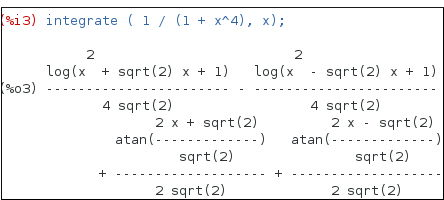
\includegraphics[height= 2cm]{ucarecdn}}
	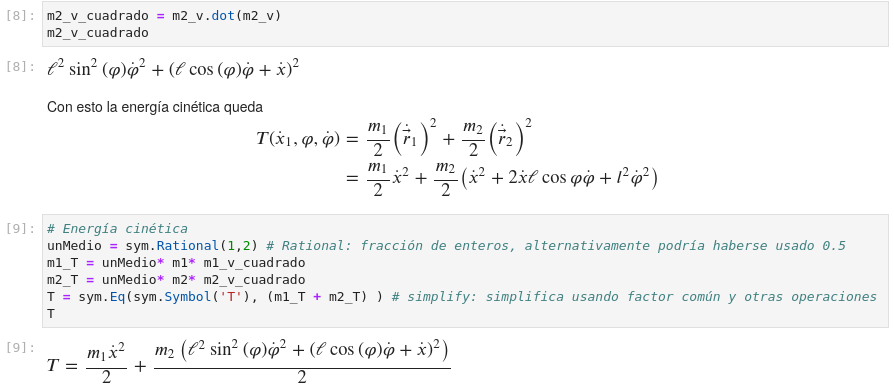
\includegraphics[width= 0.9\textwidth]{clase3sympy}
	\end{block}
	% \pause
\end{frame}


\begin{frame}
	\frametitle{Tools | 4th class | Equations for Lagrangian dynamics}
	% \pause
	\begin{block}{}
		% \uncover<4->{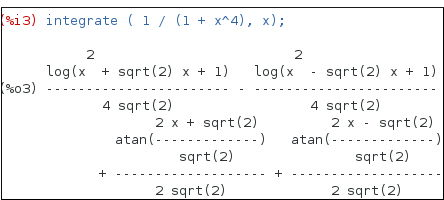
\includegraphics[height= 2cm]{ucarecdn}}
	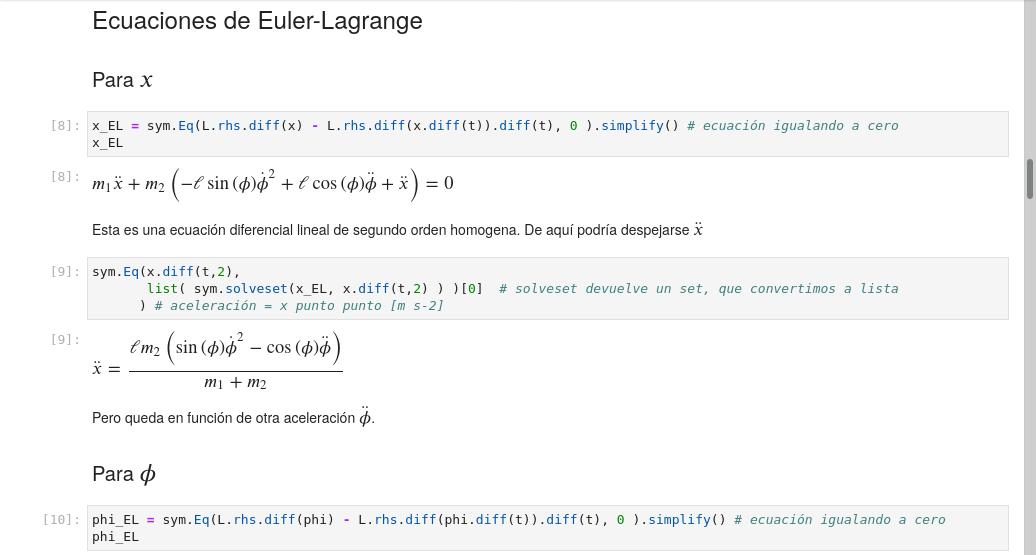
\includegraphics[width= 0.9\textwidth]{clase5EulerLagrange.png}
	\end{block}
	% \pause
\end{frame}


\begin{frame}
	\frametitle{Tools | 4th class | Automatation of resolutions}
	% \pause
	\begin{block}{}
		\begin{itemize}
			% \item No heavy calculations consuming the energy of the students.
			\item Mathematical complexity doesn't limit the scope of tackled mechanical problems.
		\end{itemize}
		% \uncover<4->{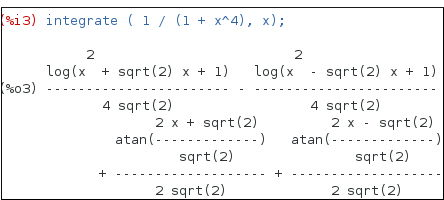
\includegraphics[height= 2cm]{ucarecdn}}
	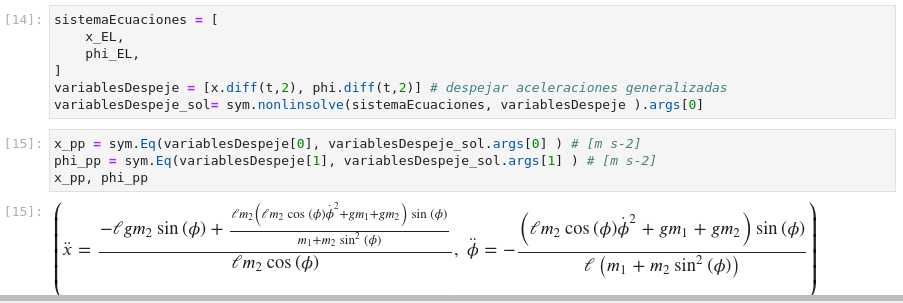
\includegraphics[width= \textwidth]{clase4Aceleraciones}
	\end{block}
	% \pause
\end{frame}


\begin{frame}
	\frametitle{Tools | 5th class | SciPy: numerical computation of results}
	% \pause
	\begin{block}{}
		%\begin{itemize}
		%	\item Explicit solutions.
		%\end{itemize}
		% \uncover<4->{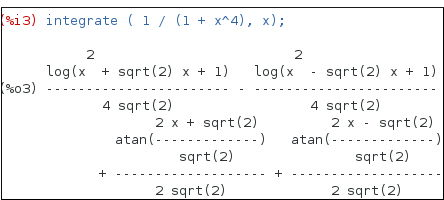
\includegraphics[height= 2cm]{ucarecdn}}
	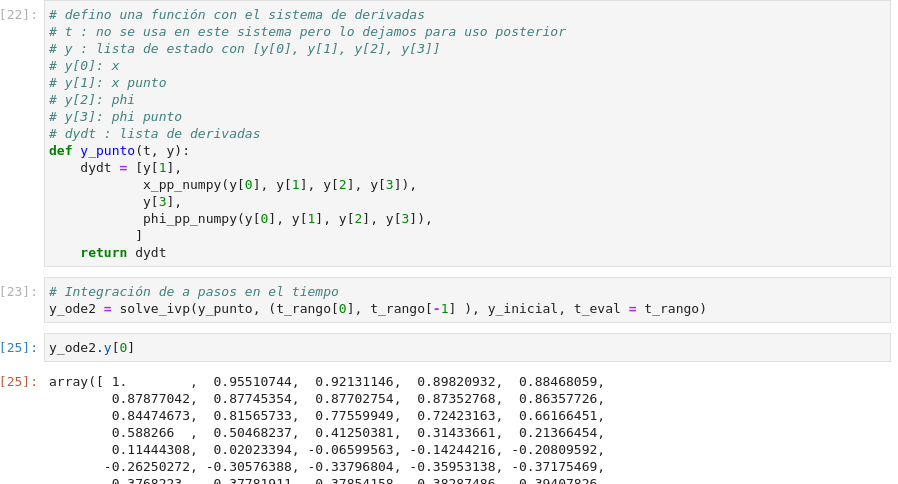
\includegraphics[width= \textwidth]{clase5Soluciones.png}
	\end{block}
	% \pause
\end{frame}


\begin{frame}
	\frametitle{Tools | 5th class | Graphical analysis of numerical results}
	% \pause
	%Class 5: analysis of results
	\begin{block}{}
		% \uncover<4->{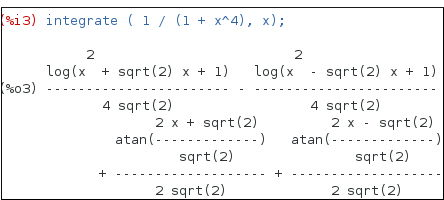
\includegraphics[height= 2cm]{ucarecdn}}
	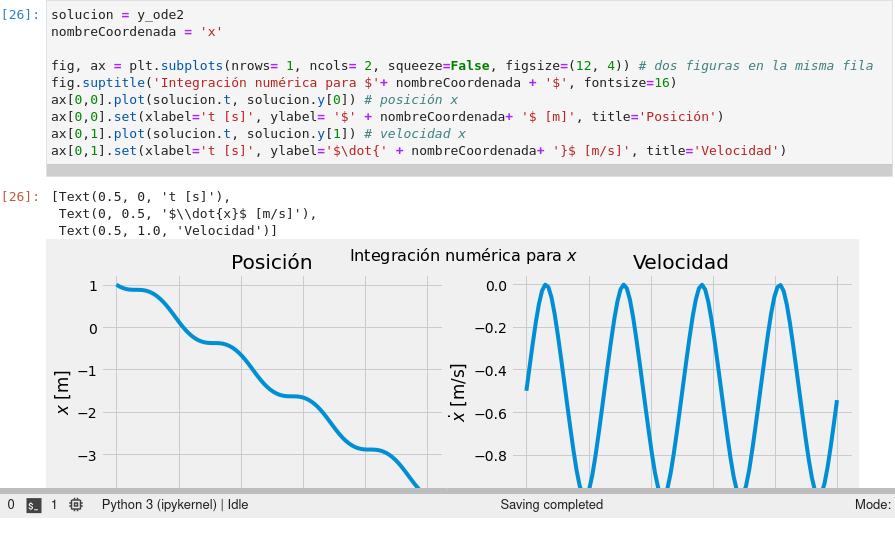
\includegraphics[width= \textwidth]{clase5Representación}
	\end{block}
	% \pause
\end{frame}

\begin{frame}
	\frametitle{Tools | 7th class | Adding complexity}
	% \pause
	%Class 7: Adding complexity
	\begin{block}{}
		\begin{itemize}
			\item Code from previous classes is \textbf{recycled} to model more realistic devices.
			%\item Gradual increase in complexity of simulated mechanical devices.
		\end{itemize}
		% \uncover<4->{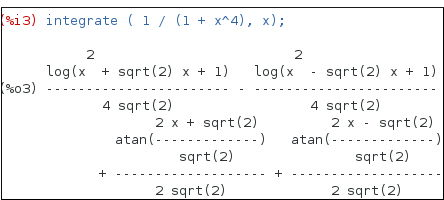
\includegraphics[height= 2cm]{ucarecdn}}
	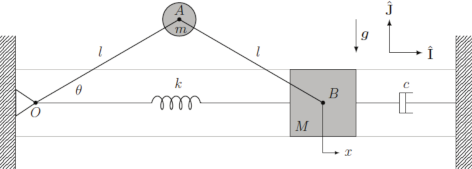
\includegraphics[height= 3.35 cm]{clase7esquema.png}
	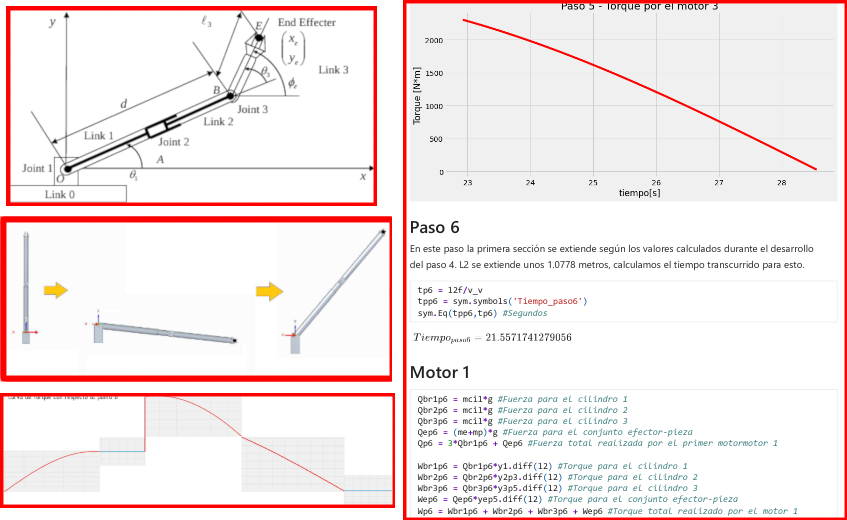
\includegraphics[height= 3.35 cm]{robotArm.png}
	\end{block}
	% \pause
\end{frame}


\begin{frame}
	\frametitle{Tools | 8th class | GitHub Copilot: AI assistance for coding}
	% \pause
	%Class 7: Adding complexity
	\begin{block}{}
		\begin{itemize}
			\item Now that the students grasp the basics they're invited to take advantage of AI
			\item After commenting in plain text what they need code is suggested
			%\item Gradual increase in complexity of simulated mechanical devices.
		\end{itemize}
		% \uncover<4->{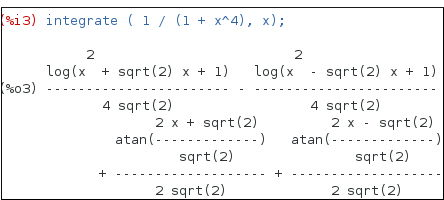
\includegraphics[height= 2cm]{ucarecdn}}
	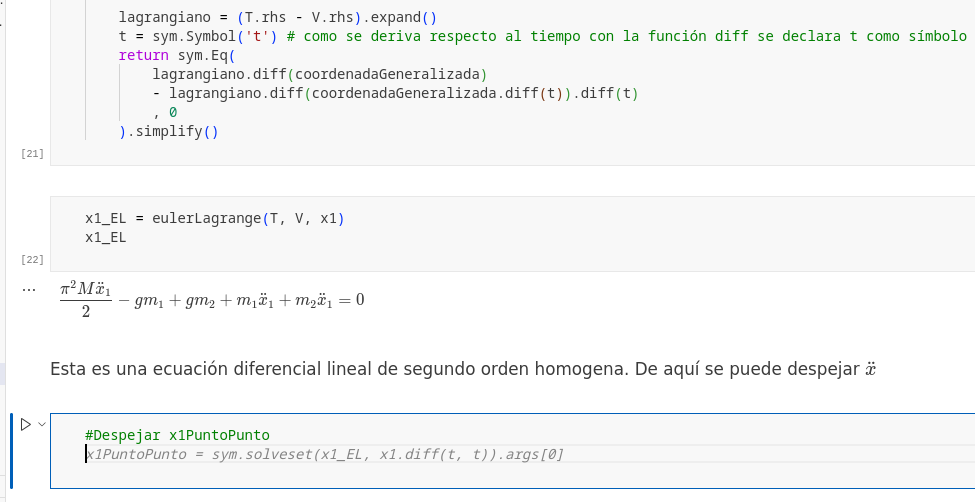
\includegraphics[width= 0.8\textwidth]{copilot}
	\end{block}
	% \pause
\end{frame}



\begin{frame}
	\frametitle{Methodology | Weekly cycle of our flipped classroom}
	\begin{block}{}
	% \begin{block}{New theory alongisde its worked examples in programmable notebooks}
		\begin{itemize}[<+->]
			\item New theory (Jupyter notebooks and videos) and assignments published on-line
			\item Previous week assignments \textbf{must} be turned-in for scoring
			\item On-line 24/7 \textbf{asynchronic} consultations that are \textbf{public} to other students
			\item \textbf{synchronic} meetings with TA's to finish assignments
%			%\item \textbf{Remote collaboration} on multi-user notebooks
			%\item Weekly meetings to \textbf{synchronically} unfinished assignments with TA's assistance
			% \item On a weekly basis these \textbf{must} be turned-in for scoring
		\end{itemize}
	\end{block}
	\begin{columns}[b]<1->
    \begin{column}{0.4\textwidth}
			\begin{block}{}
			%\begin{block}{Flipped classroom}
				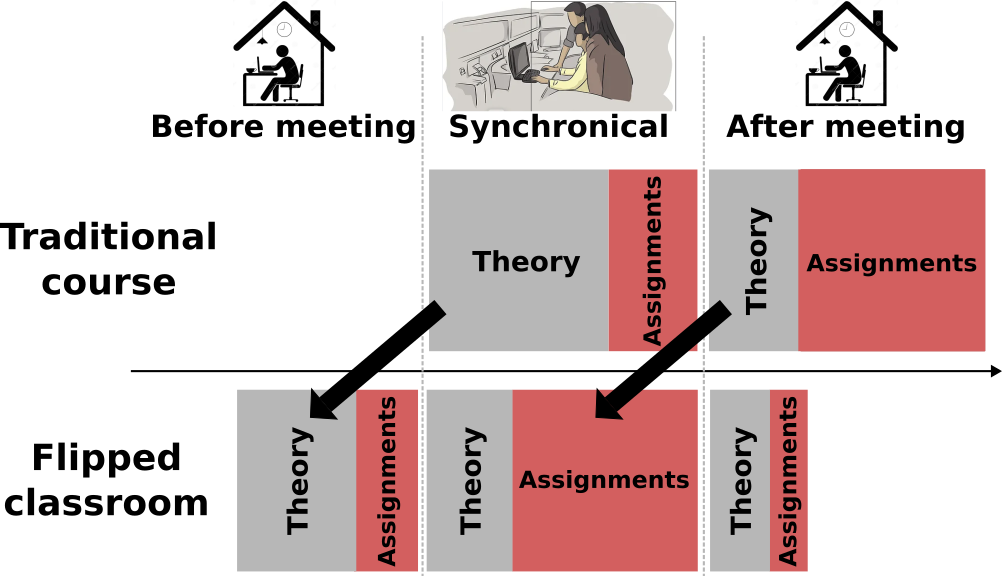
\includegraphics[width= \columnwidth]{flippedClassroomSchedule.png}
			\end{block}
    \end{column}
    \begin{column}{0.55\textwidth}
			\begin{block}{}
				\begin{tabular}{lll}
					\hline
					Synchronic & Theory & Assignments\\
					\hline
					Before & Read and apply  & Start them\\
					During & Consultations & Complete them\\
					% Durante & Aclarar dudas & \begin{tabular}{@{}c@{}}Terminarles\\(semanal)\end{tabular}\\
					After & \begin{tabular}{@{}l@{}}Additional\\consultations\end{tabular} & \begin{tabular}{@{}l@{}}TA's corrections\end{tabular}\\
					\hline
				\end{tabular}
			\end{block}
    \end{column}
  \end{columns}
\end{frame}


\begin{frame}
	\frametitle{Methodology | Google Colaboratory: asynchronic remote assistance}
	\begin{block}{}
	% \begin{block}{Student's work can be commented and edited in Google Colaboratory}
		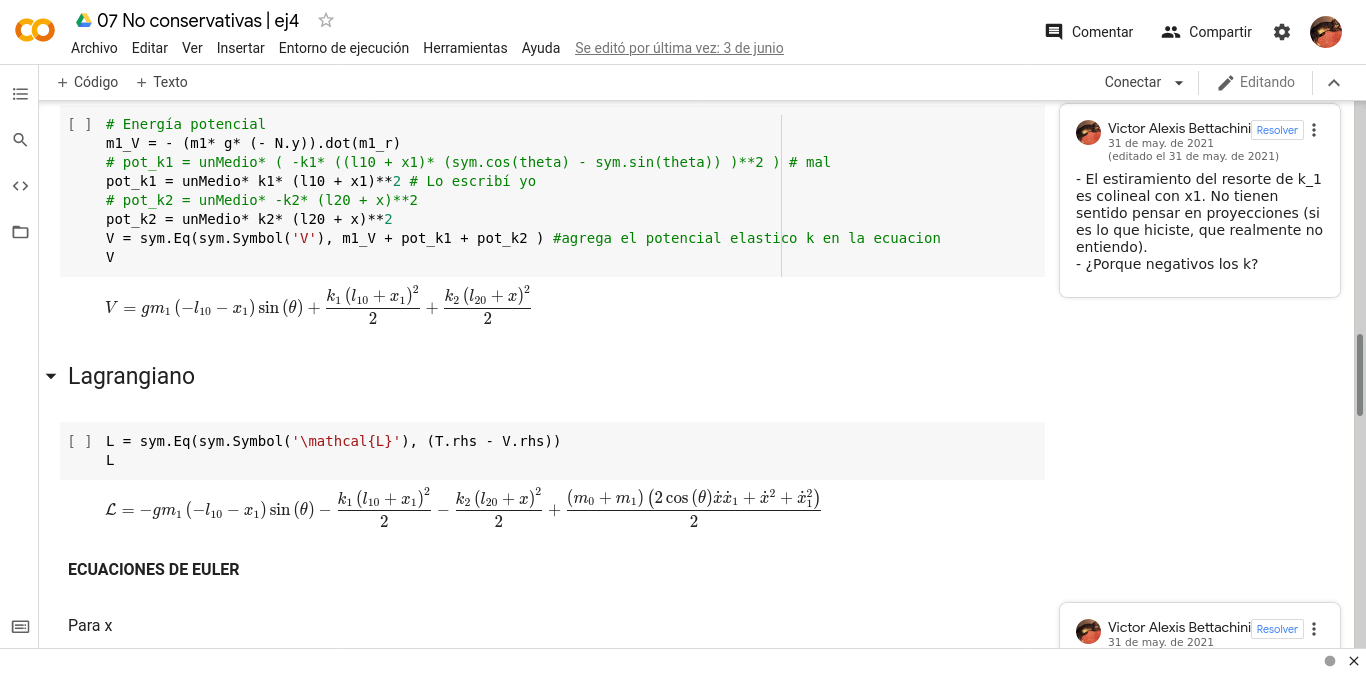
\includegraphics[width= \columnwidth]{comentariosColab}
	\end{block}
\end{frame}



\begin{frame}
	\frametitle{Methodology | Microsoft Teams: individualized student follow-up}
	\begin{block}{A record of the weekly turn-up of assignments}
		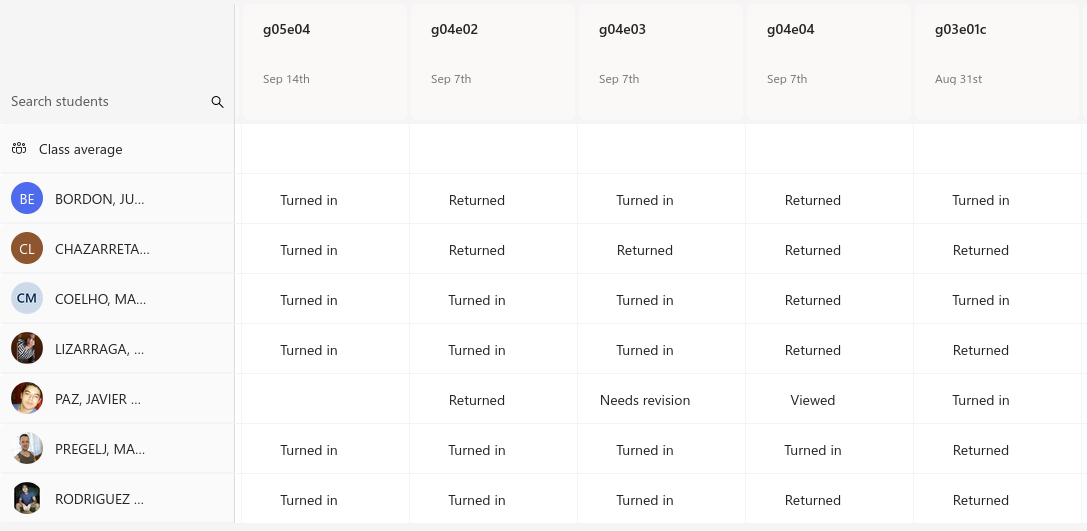
\includegraphics[width= \columnwidth]{seguimiento}
	\end{block}
\end{frame}


%\begin{frame}
%	\frametitle{Methodology | Exams are just another assignment}
%	\begin{block}{}
%	% \begin{block}{The exam is just another excercise.}
%		\begin{itemize}
%			\item The students send their notebook file.
%			\item Feedback is inserted in between the student's work.
%		\end{itemize}
%		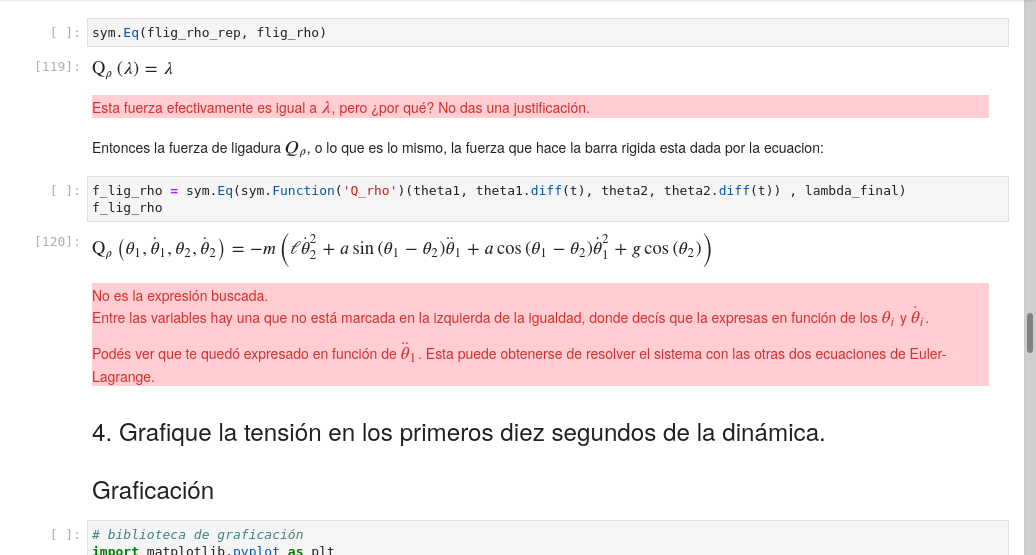
\includegraphics[width= \columnwidth]{parcial}
%	\end{block}
%\end{frame}


\begin{frame}%%     1
    \begin{center}
    \Huge Thank You!
    \end{center}
\end{frame}



\begin{frame}
	\frametitle{Summary}
	\begin{block}{A course centred on code}
		\begin{itemize}%[<+->]
			\item Material: text + equations + executable code in digital notebooks in a repository
			\item Assignments: professor's code recycling
			\item On-line:
			\begin{itemize}%[<+->]
				\item Remote collaboration and correction
				\item Doesn't require powerful nor at campus computers
				\item AI assistance for coding
				\item Dated record of each student's work
			\end{itemize}
		\end{itemize}
	\end{block}
	\begin{block}{Flipped classroom}
		\begin{itemize}%[<+->]
			\item Theory: emphasis on student's autonomus reading
			\item Reinforced by: suggested bibliography and short professor's videos
			\item Consultations: mostly on-line asynchronic and publicly accessible
			\item Synchronic mettings: TA's personal assistance for completing assignments
		\end{itemize}
	\end{block}
\end{frame}


%\begin{frame}
%	\frametitle{Course | Latest developments}
%\begin{columns}[b]
%   \begin{column}{0.47\textwidth}
%			\begin{block}{}
%				2023: student's feedback improved:
%				\begin{itemize}
%					\item Repository material: theory notes and code revised from class to class
%					\item Evaluation: grading each assignment led to a higher student's performance
%				\end{itemize}
%				2024:
%				\begin{itemize}
%					\item AI: students to code in \emph{GitHub Codespaces} with \emph{GitHub Copilot}
%					\item Translation: repository content to English (collaborations welcome!)
%				\end{itemize}
%			\end{block}
%    \end{column}
%    \begin{column}{0.48\textwidth}
%			\begin{block}{GitHub Copilot AI assists with coding}
%			%\begin{block}{Flipped classroom}
%				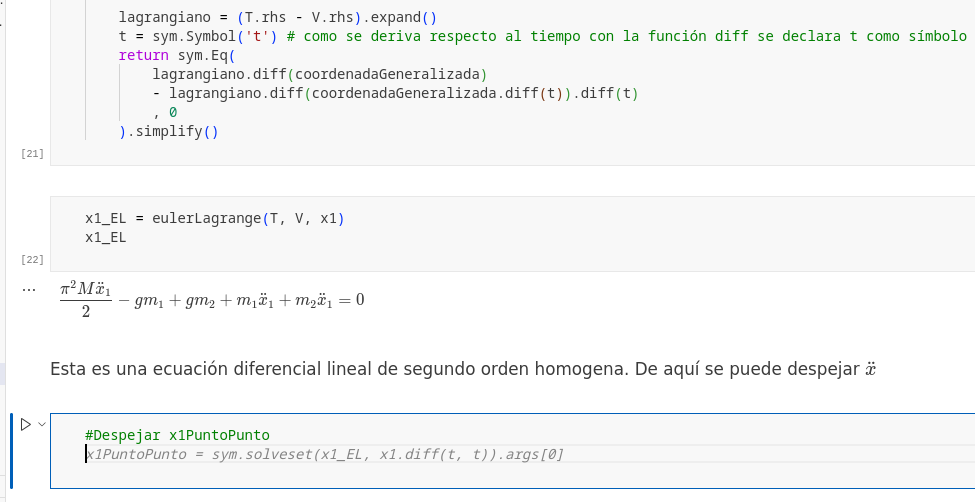
\includegraphics[width= \columnwidth]{copilot}
%			\end{block}
%    \end{column}
%	\end{columns}
%\end{frame}


%\begin{frame}
	%\frametitle{Course | Current and next steps}
	%% \pause
	%\begin{block}{}
		%\begin{description}[<+->]
			%\item [2023] Students feedback improved:
				%\begin{itemize}
					%\item Repository material: theory notes and code revised from class to class
					%\item Evaluation: grading each assignment led to a higher student's performance
				%\end{itemize}
			%\item [2024]
				%\begin{itemize}
					%%\item A course on optics and waves will incorporate part of the methodology
					%\item AI assistance in code generation by \emph{GitHub Copilot} on \emph{GitHub Codespaces}
					%\item Translate repository content to English (collaborations welcome!)
				%\end{itemize}
			%% \item [202x] Difundir la metodología en el DIIT.
		%\end{description}
	%\end{block}
	%\uncover<6->{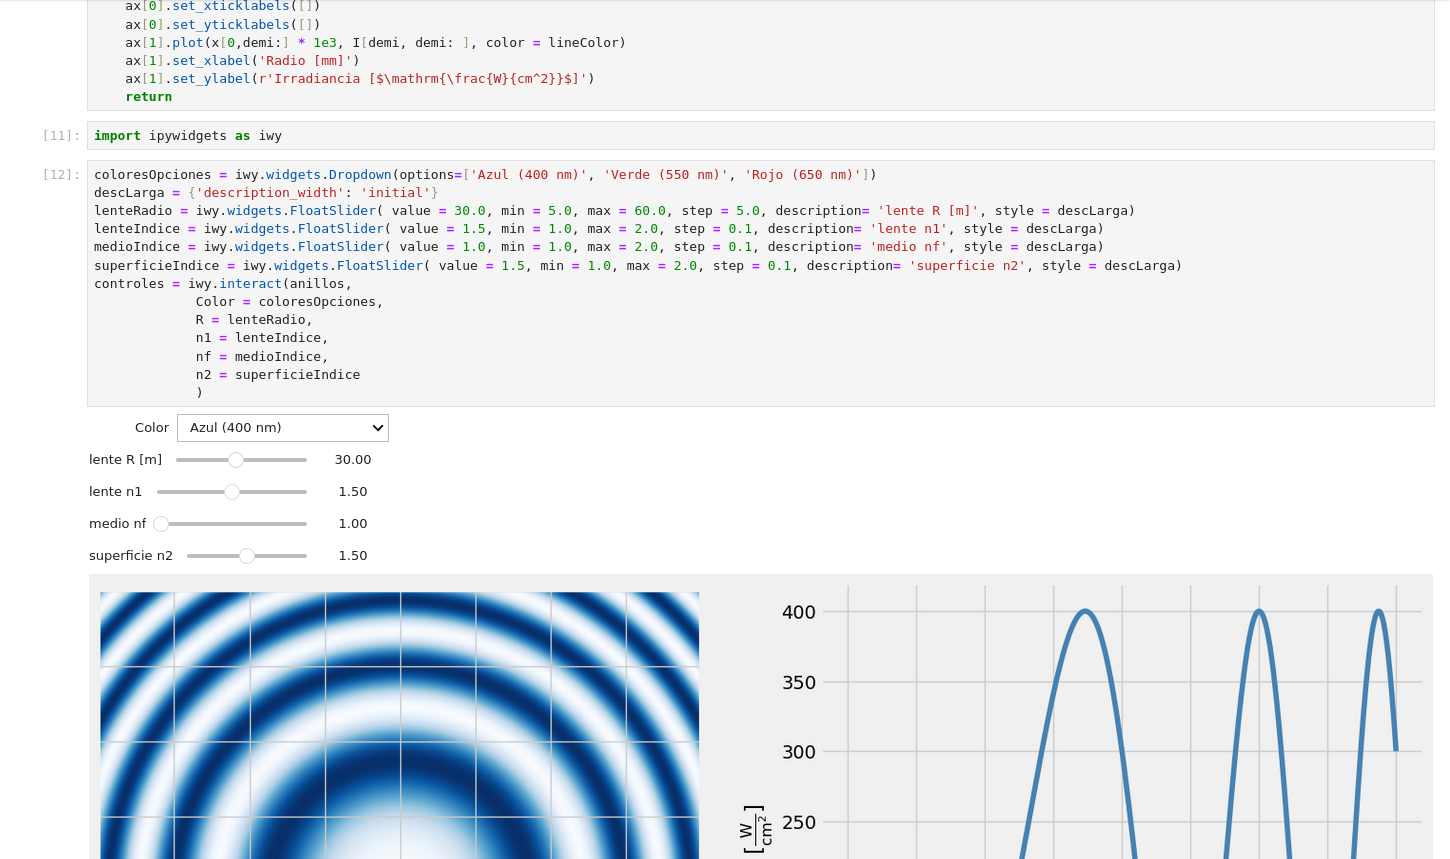
\includegraphics[height= 3.5cm]{cuñaAnillosN}}
	%\uncover<7->{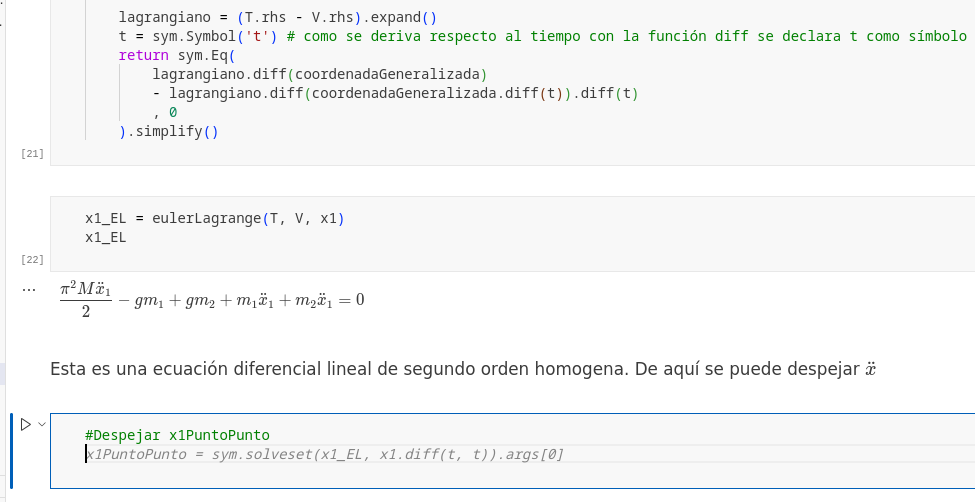
\includegraphics[height= 3.5cm]{copilot}}
%\end{frame}


\end{document}
